\documentclass[a4paper]{article}
\usepackage[utf8]{inputenc}
\usepackage[T1]{fontenc}
\usepackage[pdftex]{graphicx}
\usepackage{fancyhdr}
\usepackage{lscape}
\usepackage{color}
\usepackage{qtree}
\usepackage[english]{babel}
\usepackage{graphicx}
\usepackage[colorinlistoftodos]{todonotes}
\usepackage{listings}
\usepackage{color}
\usepackage{changepage}
\usepackage[margin=1in]{geometry}
\definecolor{codegreen}{rgb}{0,0.6,0}
\definecolor{codegray}{rgb}{0.5,0.5,0.5}
\definecolor{codepurple}{rgb}{0.58,0,0.82}
\definecolor{backcolour}{rgb}{0.95,0.95,0.92}
\usepackage[parfill]{parskip}
 \usepackage{ragged2e}
 \lstdefinestyle{mystyle}{
 	backgroundcolor=\color{backcolour},   
 	commentstyle=\color{codegreen},
 	keywordstyle=\color{magenta},
 	numberstyle=\tiny\color{codegray},
 	stringstyle=\color{codepurple},
 	basicstyle=\footnotesize,
 	breakatwhitespace=false,         
 	breaklines=true,                 
 	captionpos=b,                    
 	keepspaces=true,                 
 	numbers=left,                    
 	numbersep=5pt,                  
 	showspaces=false,                
 	showstringspaces=false,
 	showtabs=false,                  
 	tabsize=2
 }
 
\lstset{
	style=mystyle,
	inputencoding=utf8,
	extendedchars=true,
	literate={á}{{\'a}}1 {ã}{{\~a}}1 {é}{{\'e}}1,
	escapechar=\&
}
\title{Algorithmique et structures de données : Mission 3}
\date{24 octobre 2014}
\author{Groupe 1.2: Ivan Ahad - Jérôme Bertaux - Rodolphe Cambier \\ 
	Baptiste Degryse - Wojciech Grynczel - Charles Jaquet}



\begin{document}
\maketitle

\paragraph*{Question 1 (Charles Jacquet)}
\begin{itemize}
\item{\textbf{Les clés doivent-elles automatiquement être des nombres}}\\
Non, elles peuvent être n'importe quoi tant que c'est comparable.
Par exemple, ça pourrait être des String classé de manière alphabétique.
\item{\textbf{Enumérer en ordre croissant toute les clés mémorisées}}\\
il suffit d'utiliser une fonction récursive, qui va se réappeller à chaquer élément de telle sorte que :
String s = recursiveFunction(tree);

avec comme pseudo code
\begin{verbatim}
public String recursiveFunction(BinaryTree tree){
		if (tree.left == null && tree.right == null){
			return tree.getElem();
		}
		else if(tree.left == null){
			return recursiveFunction(tree.right);
		}
		else if(tree.right == null){
			return recursiveFunction(tree.left);
		}
		else{
			return recursiveFunction(tree.left) + recursiveFunction(tree.rigth);
		}
}
\end{verbatim}
La complexité de cette méthode est en O(h) avec h la hauteur du root.

\item{\textbf{Dans le cas où une clé est mémorisée deux fois}}\\
Lors de la deuxième mémorisation, dans le livre il est marqué qu'elle remplace la première. Il n'y a donc pas de relation père-fils.

\end{itemize}
\paragraph*{Question 2}
\paragraph*{Question 3 (Bertaux Jérôme)}
\begin{verbatim}
/*
* PRE : t est un arbre trié de manière croissante depuis le sous arbre de gauche vers le sous arbre de droite.
* POST : l'entrée possédant la plus petite clé ou null si l'arbre est vide.
* 
* La complexité est de l'ordre de O(h)
*/
public Entry firstEntry(Tree t){
	if(t.isEmpty()){
		return null;
	}else{
		Tree tmp = t;
		while(t2.hasLeft()){
			t2 = t2.getLeft();		
		}
		return t2.getValue();	
	}
}

/*
* PRE : t est un arbre trié de manière croissante depuis le sous arbre de gauche vers le sous arbre de droite.
			k une clé
* POST : l'entrée possédant une clé plus grande que k ou null si elle n'existe pas.
* 
* La complexité est de l'ordre de O(h)
*/
public Entry higherEntry(Tree t, int k){
	if(!t.isEmpty()){
		if(t.getValue().getKey() > k){
			return t.getValue();		
		}else if(t.hasRight()){
			higherEntry(t.getRight(), k);		
		}	
	}else{
		return null;	
	}
}
\end{verbatim}

\paragraph*{Question 4}
\newpage
\paragraph*{Question 5 (Wojciech GRYNCZEL)\\}
\textbf{L’ordre d’insertion des clés dans un AVL a t-il une influence sur la forme finale de l’arbre ?}
L’ordre d’insertion n’influence pas toujours la forme finale de l’arbre. Par exemple si on insère  les clés  (1) (2) (3) dans n’importe quel ordre, la forme finale sera toujours même: \\
\begin{center}
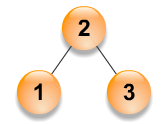
\includegraphics{tree1}
\end{center}

Mais si on insère plus de clés, la forme finale change.\\
\begin{center}
(2) (5) (6) (13) (15) (48) (1)\\
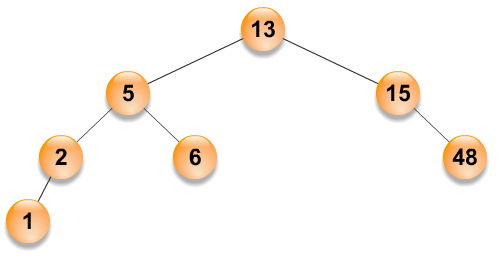
\includegraphics{tree2}\\
(1) (48) (15) (13) (6) (5) (2)\\
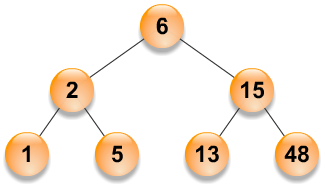
\includegraphics{tree3}
\end{center}
\newpage
\textbf{Dessinez un arbre AVL de hauteur 5 ayant un nombre minimal de nœuds :}\\
\begin{center}
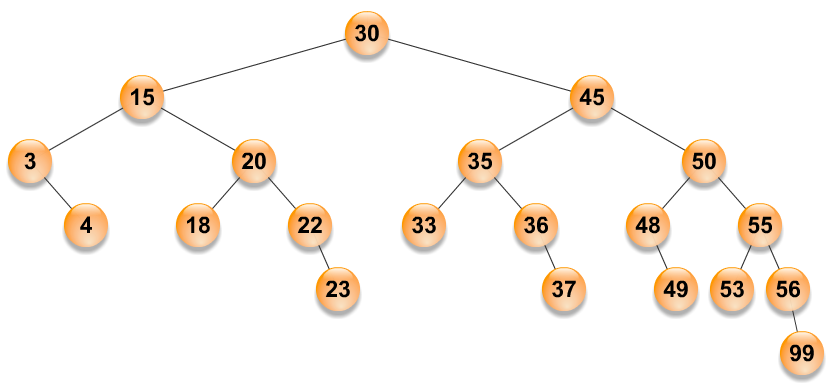
\includegraphics[scale=0.8]{tree4}
\end{center}
\textbf{Que peut-on dire de la relation entre hauteur h et nombre de noeuds n dans un arbre AVL ?}\\
La hauteur est toujours logarithmique en fonction de la taille de l’arbre.

{\footnotesize Soucres : \\
http://pauillac.inria.fr/~maranget/X/421/poly/arbre-bin.html\\
http://www.qmatica.com/DataStructures/Trees/AVL/AVLTree.html\\
http://pegasus.cc.ucf.edu/~fgonzale/eel4851/avltrees.PDF\\}

\paragraph*{Question 6}
\paragraph*{Question 7}
\paragraph*{Question 8}


\end{document}
